\documentclass[oneside]{book}
\usepackage[utf8]{inputenc}
\usepackage{float}
\usepackage{graphicx}
\usepackage{amsmath}
\usepackage{ragged2e}
\title{Notes de Cours INF 8215}
\date{2017-10-10}
\author{Olivier Sirois}
\makeindex

\begin{document}
\pagenumbering{gobble}
\maketitle
\newpage


\section{Introduction}
\paragraph{}
Ce cours est une introduction au concepts d'intelligence artificielle. On commence d'abord par aborder comment on définirait une intelligence et comment on pourrait la quantifier.
\paragraph{}
l'intelligence n'est pas unidimensionnelle. On peut remarquer certains types comme:
\begin{itemize}
\item raisonnement déductif
\item intelligence émotionnelle
\item intelligence spatiale
\end{itemize}
Ces types sont de différentes amplitudes pour chaques personnes. C'est un peu ce qui rend les gens uniques

\paragraph{}
Le génie en IA, c'est de rendre nos créations intelligentes en ce basant sur ces concepts. On joue avec ces différents types pour que nos créations puisse faire ce que l'on désire, c-à-d un comportement intelligent.
\paragraph{ex:}
Nos calculatrices sont fortes en math, GPS en navigations spatiale, etc.
\paragraph{}
L'intelligence artificielle s'est attribuer différentes définitions a travers le temps...
\subparagraph{McCarthy 1955}
Le but d’AI est de développer des machines qui se comportent
comme si elles étaient intelligentes.
\subparagraph{Brittanica 1991}
IA est la capacité d’un ordinateur numérique ou d’un robot
d’effectuer des tâches associées, à date, à des êtres intelligents.
\subparagraph{Rich 1983}
L’IA est l’étude de comment faire que les ordinateurs réalisent de
tâches pour lequelles les gens, à date, les réalisent mieux.
\paragraph{Véhicule Braitenberg}
Un concept émit par Braitenberg qui dit qu'on peut incorporer des comportements très intelligents avec des commandes très simples.
\subparagraph{Ex: voir \ref{fig:Braitenberg}}
	\begin{figure}[!ht]
		\centering
		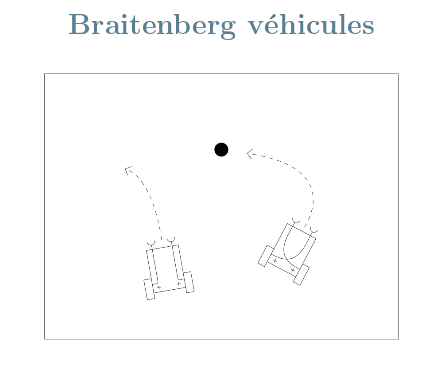
\includegraphics[width=10cm, height=10cm, keepaspectratio]{Braitenberg.png}
		\caption{Véhicule Braitenberg.}
		\label{fig:Braitenberg}
	\end{figure}
\paragraph{}	
On peut voir à travers les âges, que plusieurs civilisations (Grecques, Chine, Égypte) on modélisé leur technologies comme leurs esprits. Horloges, Systèmes hydrauliques, systèmes téléphonique, hologrammes, ordinateur analogues sont tous des métaphores de l'intelligence humaines.

\paragraph{}
Voici plusieurs événements en ordres chronologiques qui sont très important a l'IA avec une petite descriptions.
\begin{itemize}


\item \textbf{Hobbes, 1588-1679}
`Grand-Père` de l'IA. la pensée est un raisonnement symbolique. Ces idées ont été poussés par Descartes, Spinoza, Leibniz

\item \textbf{Babbage, 1792-1871}
Machine analytique, premier design d'ordinateur general-purpose

\item \textbf{Thèse Church-Turing}
Toute fonction arithmétique peut être fait sur une machine de Turing ou en calculus lambda ou formes équivalentes. n'a pas encore été prouvé mais a été testé par le temps..
\item \textbf{McCulloch et Pitts, 1943}
on prouver qu'un thresholding simple pouvait être interpréter comme une neuronne. Ce qui pourrait être une base pour une machine Turing-complete.
\item \textbf{Samuel, 1952}
Programme qui joue au checkers
\item \textbf{Minsky, 1952}
apparition du concept de réseaux de neuronnes
\item \textbf{Newell et Simon, 1956}
Programme qui trouve des preuves en logique propositionnelle.

\item \textbf{Rosenblatt, 1958}
Premier travaux significatif sur le perceptron
\item \textbf{Bobrow, 1967}
STUDENT, programme qui peut résoudre de l'algèbre de niveau secondaire en language naturel

\item \textbf{1970-1980}
Beaucoup d'effort dans les \textbf{Systèmes experts}, qui ont pour but d'avoir beaucoup de connaissances de pointes dans un domaine en particulier, pour qu'un ordinateur puisse faire des tâches de manière autonomes.
\item \textbf{Winograd, 1972}
SHRDLU, système qui peut faire une discussion et faire des actions intelligentes dans un monde simulé en utilisant que du language naturel.
\item \textbf{Warren et Pereira, 1982}
CHAT-80, peut répondre a des questions de nature géographiques en language naturel.
\item \textbf{Buchanan et Feigenbaum, 1965-1983}
DENDRAL, programme qui propose des structure atomique plausibles pour des nouveau composés organiques
\item \textbf{Buchanan et Shortliffe, 1984}
MYCIN, programme qui fait le diagnostique de maladie infectieuse du sang, prescrit le médicament requis et explique sont raisonnement
\item \textbf{1980 plus ou moins}
arrivé du prolog
\end{itemize}
\section{Agents Intelligents}
l'IA sert a utiliser un raisonnement pour faire un action. Une amalgamation d'une méthode de perception, d'un raisonnement et d'un mécanisme d'action est un \textbf{agent}. Un agent agit dans un \textbf{environnement}, les deux se trouvant dans un \textbf{monde}.
\begin{figure}[!ht]
\centering
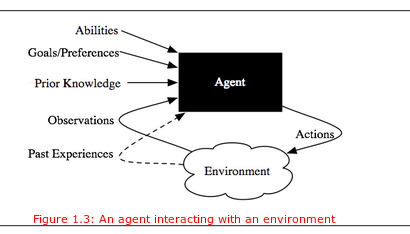
\includegraphics[width=5cm, height = 5cm, keepaspectratio]{Agent_base.png}
\caption{version generale d'un agent.}
\label{fig:Agentbase}
\end{figure}
\paragraph{}
Par exemple, un agent peut être un robot, son système de perception sont ces capteurs, sont processeur serait sa méthode de raisonnement et ses actuateurs serait sa méthode de mécanisme d'action. Son environnement serait son emplacement physique.Voici les différents types d'agents:

\begin{figure}[!ht]
\centering
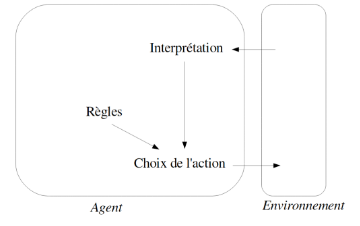
\includegraphics[width=5cm, height=5cm, keepaspectratio]{Agent_Reflexe.png}
\caption{Agent Réflexe}
\label{fig:agentreflexe}
\end{figure}
	

\begin{figure}[!ht]
\centering
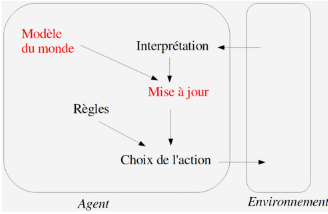
\includegraphics[width=5cm, height=5cm, keepaspectratio]{Agent_Memoire.png}
\caption{Agent Mémoire}
\label{fig:agentmem}
\end{figure}
	
\begin{figure}[!ht]
\centering
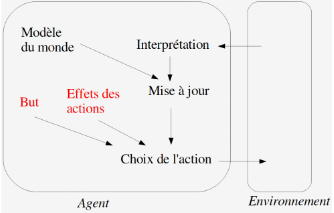
\includegraphics[width=5cm, height=5cm, keepaspectratio]{Agent_Memoire_But.png}
\caption{Agent Mémoire avec Buts}
\label{fig:agentmembut}
\end{figure}
	
\begin{figure}[!ht]
\centering
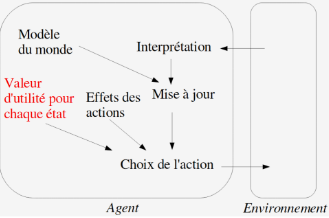
\includegraphics[width=5cm, height=5cm, keepaspectratio]{Agent_Memoire_Theorie.png}
\caption{Agent avec Théorie de la décision}
\label{fig:agenttheorie}
\end{figure}
\paragraph{}
Les agents qui peuvent apprendre sont d'une intérêt particulier. Ils peuvent eux-même changer leur comportement en fonction des échantillons d'entrainement grâces à des rétroactions positives et négatives.
\section{Méthodes de Recherche dans un Espace États}
\paragraph{État}
ou dans le monde se retrouve l'agent dans sa recherche pour la solution. C'est en fonction de chaque problême. On utilise souvent une forme arborescent pour représenter sa position.
\begin{figure}[!ht]
\centering
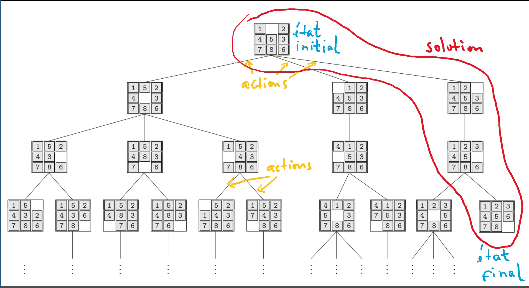
\includegraphics[width = 7cm, height = 7cm, keepaspectratio]{Etat.png}
\caption{Représentation d'un État}
\label{fig:etat}
\end{figure}

\paragraph{Fonction de Cout}
Normalement, on ne s'intéresse pas seulement a trouver une solution. On s'intéresse aussi a la qualité de la solution. On représente cela avec une fonction de cout. La convention est que le plus faible est la fonction de cout, le meilleur est la solution. Cette fonction associe une valeur a chaque action.

\paragraph{Méthode de recherche}
On définit une méthode de recherche comme étant le guideline qu'on utilise dans notre algorithme pour se déplacer dans notre espace d'états


\subsection{Méthodes de Recherche non informée}

\subsubsection{Méthode de Recherche en largeur}

\paragraph{}
La méthode de recherche en largeur cible a explorer toutes les noeuds possible de notre espace d'états sans prendre en considération la fonction de cout. Et en explorant toute les états de chaques étages de notre Arbre. Voir \ref{fig:Recherche_en_largeur} et \ref{fig:Algo_Recherche_en_largeur}

\begin{figure}[!ht]
\centering
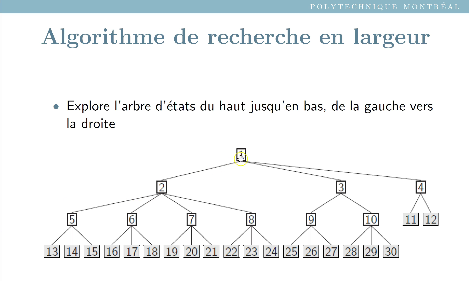
\includegraphics[width = 7cm, height = 7cm, keepaspectratio]{Recherche_Largeur.png}
\caption{Ordre d'exploration de la recherche en largeur.}
\label{fig:Recherche_en_largeur}
\end{figure}

\begin{figure}[!ht]
\centering
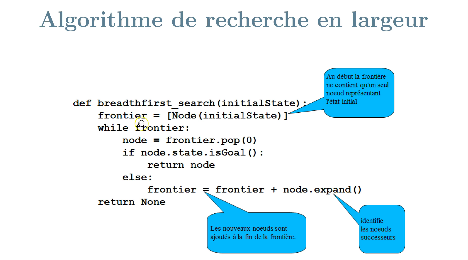
\includegraphics[width = 7cm, height = 7cm, keepaspectratio]{algo_largeur.png}
\caption{Algorithme de Recherche en Largeur.}
\label{fig:Algo_Recherche_en_largeur}
\end{figure}
\paragraph{Avantages}
on est sur d'avoir une solution. Et si tous les actions on le même cout, la solution sera optimale
\paragraph{Désavantages}
Le nombre d'état dans la frontière est très élevés.. Très grand temps de calculs et beaucoup de mémoire requis. On peut aider le problème de mémoire en prenant en considération les états déjà explorés

\subsubsection{Méthode de Recherche en profondeur}
\paragraph{}
La méthode de recherche en profondeur cible a expandre un noeud jusqu'à ce que l'état ne produit plus de nouvelle état ou qu'on trouve la solution. Si on arrive au fond. On change de branche et on commence a explorer un peu plus en largeur. Voir\ref{fig:Recherche_en_profondeur} et \ref{fig:Algo_Recherche_en_profondeur}

\begin{figure}[!ht]
\centering
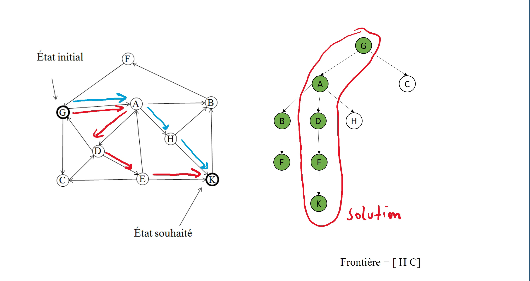
\includegraphics[width = 7cm, height = 7cm, keepaspectratio]{Recherche_Profondeur.png}
\caption{Recherche en Profondeur}
\label{fig:Recherche_en_profondeur}
\end{figure}

\begin{figure}[!ht]
\centering
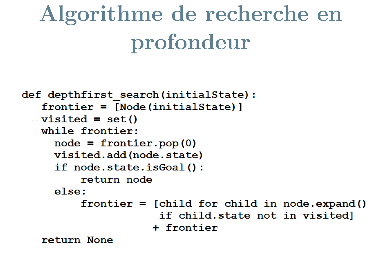
\includegraphics[width = 7cm, height = 7cm, keepaspectratio]{algo_profondeur.png}
\caption{Algorithme de Recherche en Profondeur}
\label{fig:Algo_Recherche_en_profondeur}
\end{figure}
\paragraph{Variantes Incrémentales}
On peut modifier l'algorithme de recherche en profondeur pour rectifier certains problèmes. Un des problèmes principales qu'on veut résoudre est que la recherche en profondeur peut se perdre dans une mauvaise ramification. On peut résoudre sa avec une approche incrémentale. C'est à dire, qu'on limite les solution qu'on explore en fonction de leur niveau.
\paragraph{}
Principale, on applique la recherche en profondeur avec des limites de profondeur de 1,2,3..n jusqu'à temps qu'on réussise a trouver notre solution. Sa évite que dans l'occurence qu'un problème à une très grande profondeur, qu'on se perd dans une super grande branche qui risque de ne pas donner de solution.
\paragraph{}
Cette solution n'est pas inefficace comme on l'imaginerait.. Cela est du au fait que la grande majorité du travail est fait lors du dernier niveau de l'arbre. Voir formule ci-dessous
\begin{align*}
N_{b}(D) &= \sum^D_{d=0} b^d = \frac{b^{D+1}-1}{b-1}
\end{align*}

\begin{itemize}
\centering
\item {b est le facteur de ramification}
\item {D est la profondeur de l'arbre}
\item {Nb est le nombre total de noeuds}

\end{itemize}

\subsubsection{Algorithme de Recherche a cout uniforme}

\paragraph{}
Les méthode de recherches en profondeur et en largeur ont tous les deux de grands désavantages qui rendent ces méthodes inutiles pour certains problèmes spécifiques. De plus, les deux algorithmes ne trouvent pas nécessairement la solution optimale.

\paragraph{}
L'algorithme de recherche à cout uniforme, malgré son nom un peu confusing, prend en compte de la fonction de cout. Fonction qui n'a pas nécessairement un cout uniforme.. \\

l'algorithme va toujours vouloir chercher les noeuds ayant une somme de couts minimales. Cette méthode va toujours donner une solution optimale. Par contre, elle risque d'explorer autant de noeuds que les méthodes de recherche en profondeur et en largeur. On peut considérer la recherche en largeur comme étant un cas particulier de la recherche a cout uniforme, si et seulement si la fonction de cout est égale pour chaque actions. Voir \ref{fig:Algo_Recherche_Uniforme} et \ref{fig:Recherche_Uniforme}

\begin{figure}[!ht]
\centering
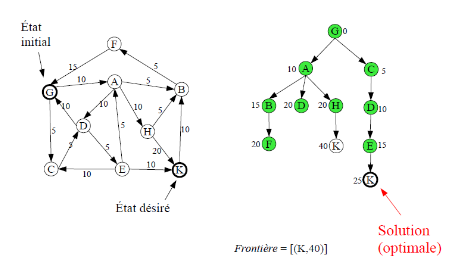
\includegraphics[width = 7cm, height = 7cm, keepaspectratio]{Recherche_Uniforme.png}
\caption{Recherche à cout Uniforme}
\label{fig:Recherche_Uniforme}
\end{figure}

\begin{figure}[!ht]
\centering
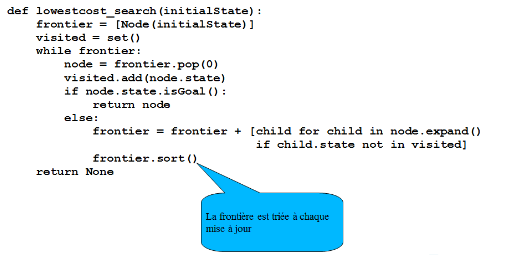
\includegraphics[width = 7cm, height = 7cm, keepaspectratio]{algo_uniforme.png}
\caption{Algorithme de Recherche a cout Uniforme}
\label{fig:Algo_Recherche_Uniforme}
\end{figure}

\subsubsection{Recherche Bidirectionel}
\paragraph{}
N'étant pas nécessairement un algorithme de recherche, la recherche bidirectionel est une facon de réduire le temps de recherche si on respect certain critères.
\begin{itemize}
\item Si on a une solution possible.
\item Si c'est possible de se rendre a la solution à partir de notre état d'origine, sinon notre solution et nos état initiale ne vont jamais converger.
\end{itemize}
 L'idée derrière la recherche bidirectionel est qu'on utilise notre algorithme de recherche dans les deux sens. Une fois en partant de l'origine pour se rendre jusqu'à la solution connus. La deuxième en partant de la solution pour essayer de se rendre jusqu'à l'état d'origine. \\
 
Normalement, on utilise une combinaison d'algorithme de recherche en profondeur partant de la solution et d'algorithme de recherche en largeur qui part de l'origine. Notre algorithme d'origine cherche a approfondire la frontière de noeud le plus largemene possible tandis que l'algorithme de notre solution cherche a la traversé. \\

Dans certains cas, nous allons avoir une amélioration. On peut la modélisé comme étant:
\begin{align*}
O_{initiale} &= b^{k} \\
O_{bidirectionel} &= 2b^{\frac{k}{2}}
\end{align*}
\begin{center}
ou b est le facteur de branchement et k la profondeur
\end{center}

\paragraph{}
Cependant, on assume toujours que nous sommes capables de rejoindre les frontières, ce qui n'est pas toujours le cas....

\subsection{Méthode de Recherche Informée}
\paragraph{Heuristique}
Une heuristique est une fonction qui essaie d'évaluer le potentiel d'un état donné en fonction de charactéristique distinctes à cet état. Ne pas confondre avec la fonction de cout, Celle-ci calcule le cout de l'état d'origine jusqu'à l'état actuel tandis que l'heuristique essaie d'estimer le cout de l'état actuel jusqu'à la solution.
\paragraph{}

par contre..
\begin{itemize}
\item Ce n'est pas garantie
\item Il faut que l'heuristique soit valide
\end{itemize}

On va s'en servir en l'incorporant dans notre algorithme de recherche, on va utiliser la fonction d'évaluation heuristique avec notre fonction de cout.\\

Pour trouver une bonne fonctions heuristiques, on peut soit parler avec un experts pour savoir quel sont les paramêtres les plus importants/qui peuvent être exploiter. \\

encore mieux, on peut aussi se servir de \textbf{l'apprentissage machine} pour pouvoir trouver nos paramêtre les plus statistiquement significatifs. Notre algorithme pourrait même ajuster son heuristique en fonction de sa.

\subsubsection{Heuristique Glutone}
\paragraph{}
Cet algorithme ne prend que l'heuristique en considération. On va s'en servir comme l'algorithme de recherche a cout uniforme sauf qu'au lieu de minimiser la fonction de cout, on va changer de voisins en prenant le voisins ayant l'heuristique la plus faible. Voir \ref{fig:Heuristique_Glutone} et \ref{fig:Prob_Heuristique_Glutone}

\begin{figure}[!ht]
\centering
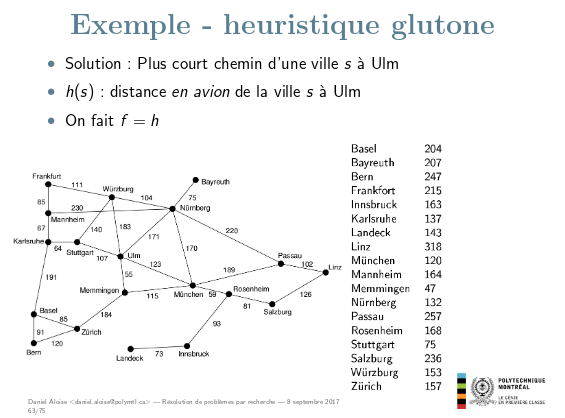
\includegraphics[width = 7cm, height = 7cm, keepaspectratio]{Heuristique_Glutone_Prob.png}
\caption{Problème d'heuristique glutone}
\label{fig:Prob_Heuristique_Glutone}
\end{figure}

\begin{figure}[!ht]
\centering
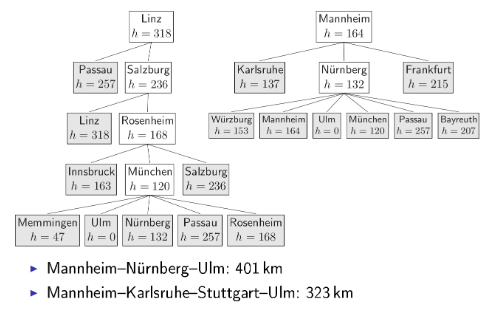
\includegraphics[width = 7cm, height = 7cm, keepaspectratio]{Heuristique_Glutone.png}
\caption{Prise de Décision de notre Heuristique Glutone}
\label{fig:Heuristique_Glutone}
\end{figure}

\subsubsection{Algorithme A*}
\paragraph{}
C'est algorithme ressemble grandement à l'algorithme de Recherche à cout uniforme. Cependant. Nous n'allons pas optimiser la fonction de cout, mais une fonction $f$ que nous allons définir comme étant
\begin{align*}
f(n) &= g(n) + h(n)
\end{align*}
\begin{center}
ou $g$ est notre fonction de cout défini dans la méthode de recherche a cout uniforme et $h$ comme étant notre heuristique. 
\end{center}


\paragraph{}
On peut alors déduire, qu'avec $h(n) = 0$ nous avons une recherche a cout uniforme et qu'avec $g(n) = 0$ nous avons une heuristique glutone. Voir fig.

\begin{figure}[!ht]
	\centering
	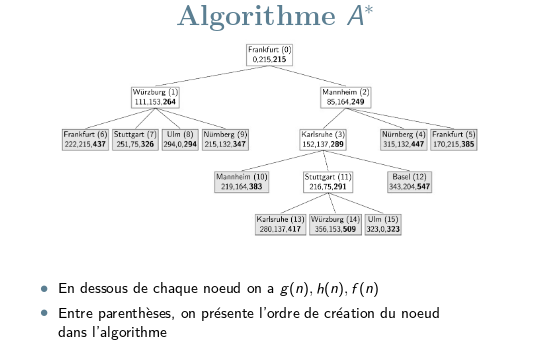
\includegraphics[width = 7cm, height = 7cm, keepaspectratio]{A*.png}
	\caption{Algorithme A*}
	\label{fig:A*}
\end{figure}
\paragraph{}
Par contre, pour que notre algorithme trouve une solution optimale, il faut que notre heuristique soit admissible. Soit:
\begin{align*}
g(x) = g(x) + h(x) \\
f(x) \leq f(z) \\
= f(x)\\
\leq f(z) \\
\leq g(z) + h(z) \leq g(y)
\end{align*}
pour fig\ref{fig:Preuve_A*}
\begin{figure}[!ht]
\centering
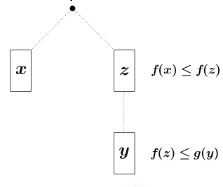
\includegraphics[width = 7cm, height = 7cm, keepaspectratio]{Preuve_A*.png}
\caption{Notre preuve pour A*}
\label{fig:Preuve_A*}
\end{figure}
\paragraph{}
Les faiblesse de l'algorithme A* sont 
\begin{itemize}
\item On peut avoir un grand nombre de noeuds à stocker
\item On doit les trier en plus à chaque itération (beaucoup de temps de calculs)
\end{itemize}
Pour régler ce problème, nous allons utiliser une recherche incrémentales.
\subsubsection{Variante A* incrémentale}
\paragraph{}
Cette variante est comme la recherche en profondeur incrémentale sauf qu'au lieu de limiter la profondeur, nous allons limiter la valeur de la fonction $f(n)$. Voir les figures 

\begin{figure}[!ht]
\centering
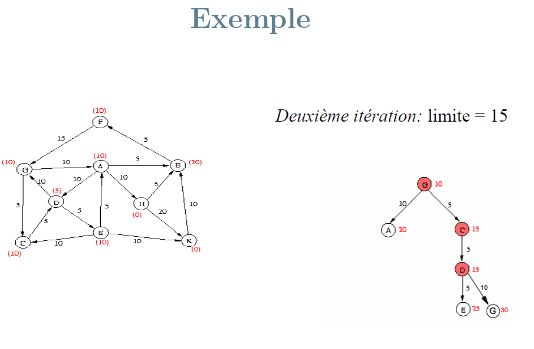
\includegraphics[width = 7cm, height = 7cm, keepaspectratio]{incrementale_15.png}
\caption{Limite de 15 dans l'approche incrémentale}
\label{fig:incrementale15}
\end{figure}

\begin{figure}[!ht]
\centering
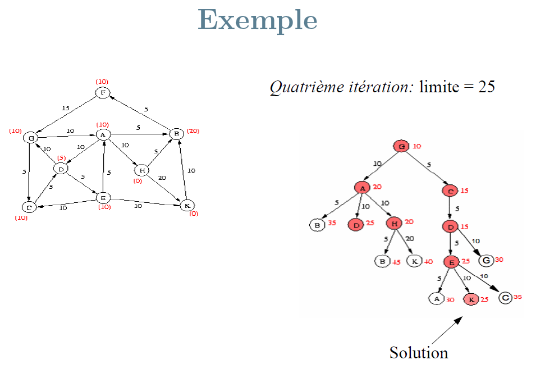
\includegraphics[width = 7cm, height = 7cm, keepaspectratio]{incrementale_25.png}
\caption{Limite de 25 dans l'approche incrémentale}
\label{fig:incrementale25}
\end{figure}
\subsection{Méthode de Recherche Locale}
\paragraph{Voisinage}
On appel un voisinage tous les noeuds qui peuvent être un successeur de l'état en question. pour revenir à notre analogie arborescente, le voisinage de l'état initiale serait l'étage en dessous. Le voisinage de tous les états du première étage serait les états du deuxième étage.. ainsi de suite.\\

Les méthodes de recherche locales ne conservent qu'un seul noeud en mémoire, celui ou nous sommes. En générale, avec une méthode de recherche locale on cherche seulement à trouver une solution, et non pas comment se rendre à la solution selon notre origine.\\

À chaque itération de notre algorithme, on remplace par notre meilleur noeuds jusqu'à temps qu'on a une solution. Normalement, on essaie de concevoir l'algorithme de sorte qu'il essaie de minimiser les conflits. Ou la solution possible est une solution sans conflit. \\

\noindent
Pour un voisinage étant défini comme un voisinage n-opt, cette fonction décrit l'ordre de complexité du voisinage.
\begin{align*}
O(n^k)
\end{align*}
\begin{center}
ou k est égale au nombre d'opérations permis
\end{center}

\paragraph{Randomisation} Si on peut trouver un bon optimum local avec un prob de $p$, une solution sera trouver en faisant $O(1/p)$ éxécutions.

\subsubsection{Recuit Stimulé}
Le problème avec les méthodes généraliste de recherche locale est qu'il n'ont pas de notions de max-min local. C'est à dire, lorsqu'il va trouver un max ou un min, il ne sera pas si c'est le max-min globale, ou si c'est juste une max-min ordinaire(locale) 
\paragraph{Fait empirique:} Les bon optima locaux sont souvent près les uns des autres.\\

l'objectif de l'algorithme de recuit sitmulé est de laisser des solution mauvaise passer. Tout sa pour pouvoir sortir des différents max-min locale (voir fig \ref{fig:paysage_espace}

\begin{figure}[!ht]
\centering
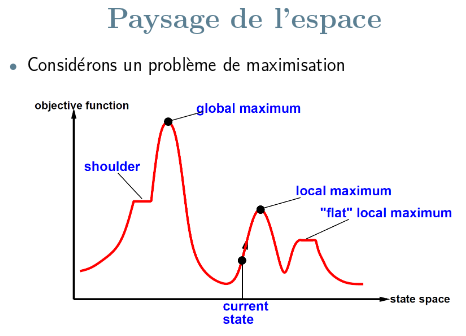
\includegraphics[width = 7cm, height = 7cm, keepaspectratio]{Paysage_Espace.png}
\caption{Exemple de Paysage de l'Espace. On cherche à trouver le maximum global sans rester pris dans un max locale}
\label{fig:paysage_espace}
\end{figure}
\paragraph{}
Au fur et à la mesure que le problème augmente en taille, le raport entre les mauvais et les bons optima locaux augmente (exponentiel). Ce qui rend le redémarrage de l'algorithme avec un départ différent futile. C'est la raison pourquoi on se sert du Recuit Stimulé. voir fig. pour algorithme.

\begin{figure}[!ht]
\centering
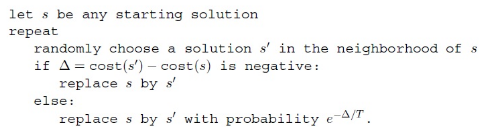
\includegraphics[width = 7cm, height = 7cm, keepaspectratio]{Recuit_Stimule.png}
\caption{Algorithme de Recuit Stimulé}
\label{fig:recuit_stimule}
\end{figure}
La difficulté avec le recuit stimulé est de trouver un bon régime de refroidissement pour T. Cet algorithme est rendu obsolete comparer a l'algorithme génétique.
\subsubsection{Algorithme Génétique}
\paragraph{}
L'algorithme génétique est très flexible. Dans le cours, il est considéré comme une recherche local tandis que certains expert le considère comme une recherche globale. \\

Le principe de l'algorithme génétique est de représenter ton problème/état comme étant une chaine de symbole (une entité). Nous avons besoin d'une quantité de solution possible, que nous allons appeller \textbf{population}. Nous essayer de répliquer la théorie de l'évolution sur cette population en appliquant des \textbf{croisements} et des \textbf{mutations}. Nous allons ensuite répéter le processus $n$ fois jusqu'à temp qu'un individu dans notre populations soit une solution qu'on désigne comme acceptable.\\

Voici les ligne directrice de l'algorithme génétique. (fig. \ref{fig:algo_genetique} et fig \ref{fig:exemple_algo_genetique} ) 

\begin{figure}[h!t]
\centering
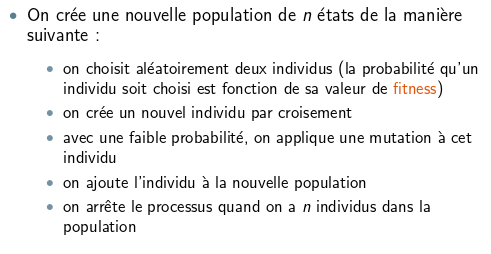
\includegraphics[width = 7cm, height = 7cm, keepaspectratio]{algo_genetique.png}
\caption{Ligne directrice de l'algo génétique}
\label{fig:algo_genetique}
\end{figure}


\begin{figure}[h!t]
\centering
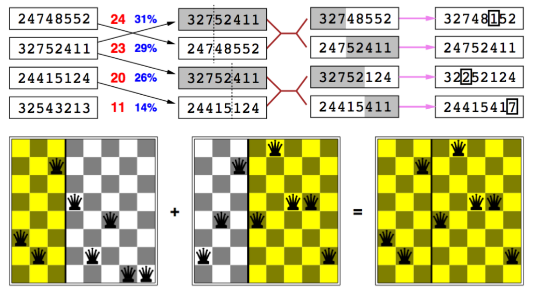
\includegraphics[width = 7cm, height = 7cm, keepaspectratio]{exemple_algo_genetique.png}
\caption{Exemple visuel d'algorithme génétique}
\label{fig:exemple_algo_genetique}
\end{figure}
\paragraph{}
L'algorithme génétique est très flexible. On peut nous même déterminer notre processus de sélection des solutions optimales après avoir fait notre croisements et mutations. On peut sélectionner pour vraiment avoir une bonne diversité génétique dans notre population ou on peut s'assurer de vraiment choisir les solutions optimales. Par contre, il faut réaliser qu'il est difficile de générer de meilleurs solutions si notre populations est hétérogènes. Alors il faut quand même s'assurer d'avoir des solutions qui ne sont pas nécessairement optimale, mais différent au point de vue du génotype.\\

voici sur la prochaine page quelques exemples d'opérateur de croisement et de mutations.
\begin{figure}[h!t]
\centering
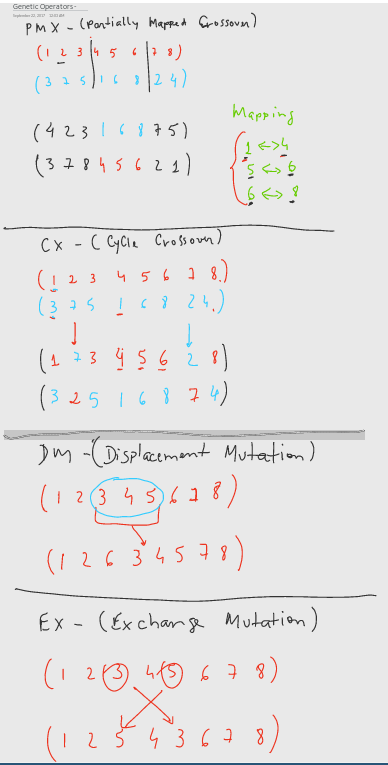
\includegraphics[height = 15cm, keepaspectratio]{operateur_genetique.png}
\caption{Exemple d'opérateurs génétiques}
\label{fig:ops_genetique}
\end{figure}
\section{Problème de Satisfaction de Contraintes}
\noindent Quoique très courte, cette section reste quand même très importante. \\
On formule un problème de satisfaction de contraintes comme suit:\\

\noindent un état est défini par $n$ variables $X_i, i = 1...n$ \\
\noindent Ces valeurs appartienne à un domaine $D_i$ \\

Cette formulation mène à la création d'algorithme généraliste. Le principe est de trouver une solution qui satisfait toute les contraintes appliquer sur les variable $X_{i\rightarrow n}$. Par contre, sa peut être utile d'analyser le problème à l'aide d'un graphe de contraintes.\\

\noindent On peut classer les contraintes par type. Ou: \\
\noindent \textbf{unaire} $\rightarrow$ s'applique à une seul variable\\
\noindent \textbf{binaire} $\rightarrow$ s'applique à deux variable\\
\noindent \textbf{ordre supérieur} $\rightarrow$ s'applique à plusieurs variables... très simple\\
\\subsection{Recherche Standard}
On défini la recherche standard comme:
\noindent \paragraph{état initiale:} l'affectation vide
\noindent \paragraph{successeurs :} affect une valeur à une variable pas affecté sans ajouter de conflits avec les affectations précédente $\rightarrow$ si ce n'est pas possible, la ramification est coupés. 
\noindent \paragraph{test de finitude :} l'affectation de variable complète.\\

c'est le même algorithme pour tous les problèmes, on suppose que le chemin pour se rendre à la solution n'est pas important. 

\begin{figure}[!ht]
\centering
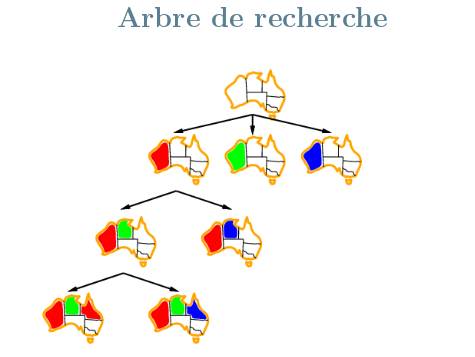
\includegraphics[width = 7cm, height = 7cm, keepaspectratio]{arbre_recherche_standard.png}
\caption{Arbre de Recherche Standard}
\label{fig:arbre_recherche_standard}
\end{figure}
\subsection{Backtracking}
Dans le cas ou notre algorithme prend une mauvaise branche par accident. On doit utiliser le backtracking pour revenir sur nos pas et pour pouvoir prendre la bonne branche.
Ce processus est inneficace. on finit par faire une recherche qui regarde une bonne partie des possibilités de notre arbre d'état. Ce qui en revient à faire une recherche en profondeur... \\
Pour pouvoir améliorer notre backtracking, on peut utiliser plusieurs méthodes.

\subsubsection{Heuristiques dans le Backtracking}
On trouve une fonction heuristique pour chaque contraintes. Sa pourrait être quelques chose qui choisit une valeur pour ta variable qui génère le moins de conflits. Sa pourrait être aussi qu'on choisit la variable qui à le plus grande nombre de contraintes et de choisit une valeur qui génère le plus de possibilité dans toutes les contraintes.

\subsubsection{Forward-checking}
C'est très self-explanatory. Le principe c'est de regarder le domaine de chaque variable instancié, et que pour chaque valeur qu'on attribuerait, on regarde si on viole une contrainte. \\

Si c'est le cas, on la retire du domaine. on s'arrète quand le domaine d'une variable est vide. Par contre, on ne peut pas détecter toute les violations (Pour pouvoir détecter toutes les violations, il faudrait faire du forward checking d'ordre du nombre de variable dans notre domaine, ce qui reviendrait à faire une recherche en largeur..) voir fig \ref{fig:forward_checking}

\begin{figure}[!ht]
\centering
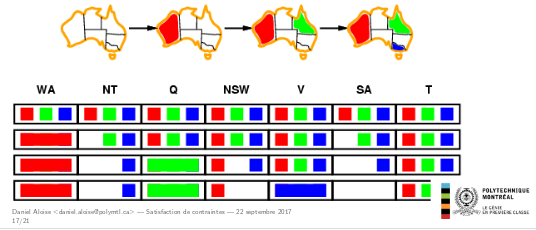
\includegraphics[width = 7cm, height = 7cm, keepaspectratio]{forward_checking.png}
\caption{Exemple de Forward Checking}
\label{fig:forward_checking}
\end{figure}

\subsubsection{Cohérence d'arc}
La dernière méthode de backtracking est la cohérence d'arc. Cette méthode en principe, regarde toute les variables et les compares avec toutes les autre variable. On compare toute les attributions de domaine, et on enleve toutes les valeur possible qui génère un conflit avec les autre valeurs de la variable à lequel tu la compare. On fait une comparaison avec toute les permutations de variables. voir fig \ref{fig:gac1}, \ref{fig:gac2}, \ref{fig:gac3} \\

\begin{figure}[!ht]
\centering
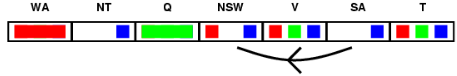
\includegraphics[width = 7cm, height = 7cm, keepaspectratio]{gac1.png}
\caption{Step1 GAC}
\label{fig:gac1}
\end{figure} 

\begin{figure}[!ht]
\centering
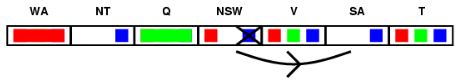
\includegraphics[width = 7cm, height = 7cm, keepaspectratio]{gac2.png}
\caption{Step2 GAC}
\label{fig:gac2}
\end{figure}

\begin{figure}[!ht]
\centering
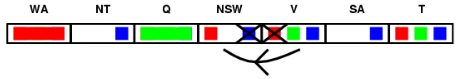
\includegraphics[width = 7cm, height = 7cm, keepaspectratio]{gac3.png}
\caption{Step3 GAC}
\label{fig:gac3}
\end{figure}

\section{Logique Propositionelle}
Apparament, en tant qu'humain on sait des choses. C'est chose pour être interpréter comme étant des connaissance sur le monde. On opère en fonction de ces connaissance et non en fonction d'un pure réflexe (voir Réseau de Neurones). On utilise un \textbf{raisonnement} basé sur nos \textbf{connaissances}. Jusqu'à dâte, nos méthode de recherches sont basé sur des problèmes très spécifiques.\\

Un Agent logique suit un framework comme suit:\\

\begin{figure}[h!t]
\centering
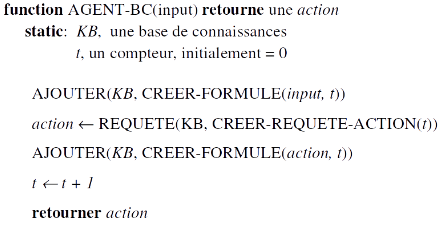
\includegraphics[width = 7cm, height = 7cm, keepaspectratio]{agent_logique.png}
\caption{Framework d'un agent Logique}
\label{fig:agent_logique}
\end{figure}

Le principe est que tu envoie la perception de ton agent dans sa base de connaissance. Ensuite en utilisant une méthode de référence, tu peux déduire certaines affirmations sur le monde. Ensuite, l'agent finit par redemander certaines affirmations sur le demande. Affirmations lequel la base de connaissance répond par un oui ou un non.\\

\noindent Un agent logique utilise:
\begin{itemize}
\item un \textbf{language formel} qui lui permet de représenter de façon compacte plusieurs situations différentes (logique propositionel et logique de premier ordre)

\item une \textbf{base de connaissances} pour stocker les faits connus spécifiques aux problèmes

\item des \textbf{algorithme d'inférence généraux} pour déduire des nouveaux faits.
\end{itemize}

\subsection{Conséquence Logique}
On définit une conséquences logique comme une chose conséquence d'un autre
\begin{align*}
KB \models \alpha
\end{align*}
\noindent est vraie si seulement si $\alpha$ est vrai dans tous les monde ou $KB$ est vrai aussi.

\noindent Exemple: $ KB = ( x = 3 ), KB \models ( x + 2 = 5 )$

On dit que $KB$ est un modèl de $\alpha$ dans la condition d'en haut.. On pourrait élaborer et dire qu'un modèle d'un affirmation $\alpha$ serait en fait une possibilité de représentation du monde.. voir fig 

\begin{figure}[h!t]
\centering
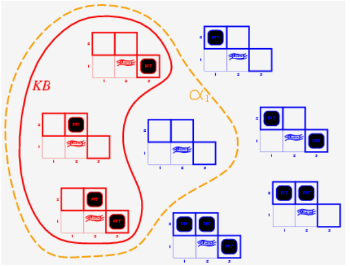
\includegraphics[width = 7cm, height = 7cm, keepaspectratio]{exemple_model.png}
\caption{Exemple d'un model}
\label{fig:exemple_model}
\end{figure}
\subsection{Syntaxe de la Logique}
la logique propositionnelle suit des règle très spécifique avec sa propre famille d'opérateur. En voici des exemples.\\

\begin{itemize}


\item Le connecteurs : $\wedge$,
$\vee$,
$\Rightarrow$,
$\Leftrightarrow$,
$\neg$ ont tous des fonctions specifiques 
\item pour S, nous avons $\neg$ S qui donne sont inverse (negation) implique $\neg$ S est vraie si S est faux
\item pour $S_1 et S_2$, on a $S_1 \wedge S_2$ si $S_1$ est vraie et $S_2$ est vraie
\item pour $S_1 et S_2$, on a $S_1 \vee S_2$ si $S_1$ est vraie ou $S_2$ est vraie
\item pour $S_1 et S_2$, on a $S_1 \Rightarrow S_2$ si $S_1$ est faux ou $S_1$ est vrai, \\
ie. c'est faux si $S_1$ est vraie et $S_2$ est faux
\item pour $S_1 et S_2$, on a $S_1 \Leftrightarrow S_2$ qui est equivalent a $S_1 \Rightarrow S_2$ et $S_2 \Rightarrow S_1$ 

\end{itemize}

Notre base de connaissance va être former d'une multitude de statements sous forme $X_1 \vee X_2 \wedge \neg X_3$ ou les variables X sont des variable qui représente certains aspects du monde. Comme par exemple sa pourrait représenter l'état d'une switch dans un circuit ou $True$ serait égale à un courant qui passe dans la switch et que $False$ serait lorsque rien ne passe dans la switch.\\


à l'aide de la syntaxe de la logique et de notre base de connaissance composés d'une multitude  de statements sur le monde. Il est possible de faire des déductions sur le monde basé que sur les statements dans notre base de connaissances.\\

On peut déduire une affirmation $\alpha$ de KB et l'écrire sous la forme : \\
\begin{center}
$ KB \vdash \alpha$
\end{center}

voici quelques règles d'inférence qui est valable:
\begin{align}
\neg(A\vee B) \vdash (\neg A\wedge \neg B) \textbf{      Loi de de Morgan}\\
\neg(A\wedge B) \vdash (\neg A \vee \neg B) \textbf{       Loi de de Morgan}\\
[(A \Rightarrow B), A] \vdash B \textbf{        Modus Ponens}\\
[(A \Rightarrow B), \neg B] \vdash \neg A \textbf{        Modus Tolens}\\
(A \wedge B) \vdash A \textbf{       Élimination du } \wedge\\
(A \Leftrightarrow B) \vdash (A\Rightarrow B) \wedge (B\Rightarrow A)\\
[(A \vee B), \neg A] \vdash B
\end{align}

\subsection{Inférence}
Pour faire de l'inférence, nous n'avons qu'à appliquer les formules vu ci-haut. On définit:
\paragraph{Algorithme de résolution :} Les formules sont normalisé et on applique une règles de résolution que nous allons voir plus bas

\paragraph{Formes Normale Conjonctive} Une formule est en FNC si et seulement si elle consiste d'une conjonction de clauses ou une clauses est une disjonction de littéraux. Un littéraux peut être vraie ou faux.
\begin{align}
FNC = K_1 \wedge K_2 \wedge K_m \\
\text{K est une clause} \rightarrow K_i = L_1 \vee L_2 \vee L_m\\
\text{ou L est un littéraux, vraie ou faux}\\
\text{forme finale = } (L_{11}\vee L_{12})\wedge (L_{21} \vee L_{22})
\end{align} 

\noindent Toute base de connaissance en Logique Propositionelle peut être traduite en Forme normale conjonction à l'aide de:\\ \\
\centering
$(A \Rightarrow B) \vdash \neg A \vee B$
\justify

\noindent On utilise ensuite la loi de De Morgan pour rendre les statements en une combinaise de $\vee$ et de $\wedge$. voir fig.\ref{fig:exemple_inference}

\begin{figure}[h!t]
\centering
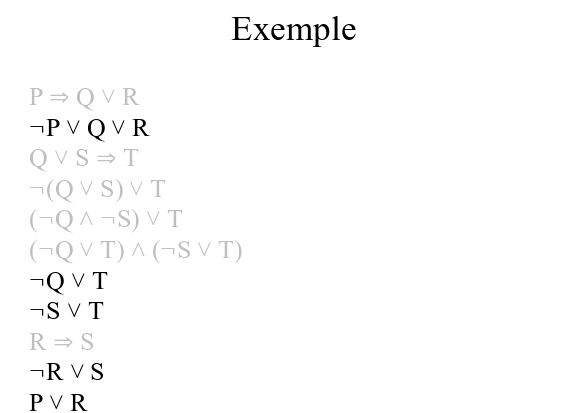
\includegraphics[width = 7cm, height = 7cm, keepaspectratio]{exemple_inference.png}
\caption{Exemple d'une traduction de statements en FNC}
\label{fig:exemple_inference}
\end{figure}

\noindent La base de connaissance KB doit toujours être consistante. c-à-d quelle ne se contredit pas elle dans ses statements. Exemple avoir un statement $S_1$ et de vouloir rajouter $\neg S_1$

\noindent Nos algorithme d'inférence peut être classifier de deux manières:

\begin{itemize}
\item \textbf{Algorithme Complet} Si un fait est une conséquence logique de la base de connaissance, notre algorithme doit être capable de déduire ce fait.\\
Si $KB \models \alpha$ alors $KB \vdash \alpha$

\item \textbf{Algorithme Correct} Si l'algorithme d'inférence déduit un fait. Celui-ci doit être nécessairement une conséquence logique de la base de connaissance, c-à-d, qu'il n'invente pas des fausseté. \\
Si $KB \vdash \alpha$ alors $KB \models \alpha$
\end{itemize}

\subsubsection{Clause de Horn}
On peut être encore plus spécifique dans notre définitions d'une clause. Les \textbf{clauses de horné} est une ensemble de clauses il y a au plus un littéral positif. voir fig \ref{fig:horn} 

\begin{figure}[h!t]
\centering
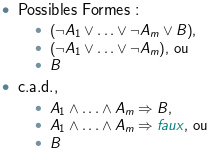
\includegraphics[width = 5cm, height = 5cm, keepaspectratio]{horn.png}
\caption{Formulation d'une clause de Horn}
\label{fig:horn}
\end{figure}

\noindent C'est important car en prolog, tout doit être défini par des clauses de horn.

\subsubsection{Chaînage Avant}
le premier algorithme d'inférence que nous allons voir est l'algorithme de chaînage avant. Le principe de l'algorithme est pouvoir déduire tout ce que nous pouvons avec notre base de connaissance, et ensuite de vérifier si nous pouvons déduire le statement que nous voulons, c-à-d $\alpha$. voir fig.\ref{fig:exemple_chainage avant} et \ref{fig:algo_chainage_avant}

\begin{figure}[h!t]
\centering
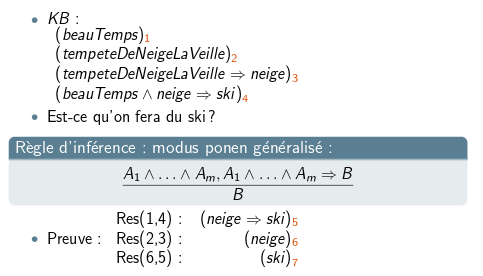
\includegraphics[width = 5cm, height = 5cm, keepaspectratio]{chainage_avant_exemple.png}
\caption{Exemple de chaînage avant}
\label{fig:exemple_chainage avant}
\end{figure}

\begin{figure}[h!t]
\centering
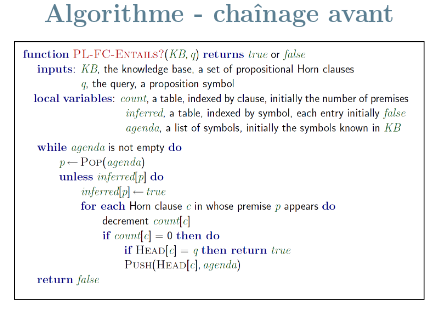
\includegraphics[width = 5cm, height = 5cm, keepaspectratio]{algo_chainage_avant.png}
\caption{Algorithme de chaînage avant}
\label{fig:algo_chainage_avant}
\end{figure}

\subsubsection{Chaînage Arrière}
Le deuxième algorithme d'inférence que nous allons voir est le chaînage arrière. cet algorithme essaie d'ajouter la négation du fait à prouver dans la base de connaissance. Si on fini avec une clause vide, sa veut dire que le fait qu'on essaie de prouver est faux (fig \ref{fig:exemple_chainage_arriere}). Il faut prendre garde. Car l'algorithme de chaînage passe les statements un à un de haut en bas. Il se peut que notre algorithme rentre dans une boucle infini si certains statements se font références (fig \ref{fig:chainage_arriere_loop}).\\

\begin{figure}[h!t]
\centering
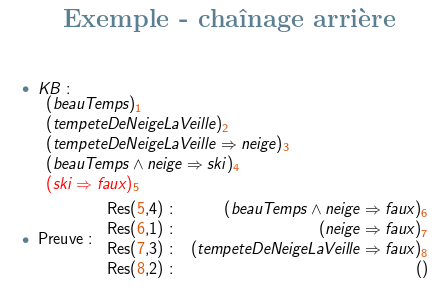
\includegraphics[width = 5cm, height = 5cm, keepaspectratio]{exemple_chainage_arriere.png}
\caption{Exemple d'un chaînage arrière}
\label{fig:exemple_chainage_arriere}
\end{figure}


\subsubsection{WalkSat}
Le troisième algorithme est le WalkSat. C'est en fait un algorithme très probabiliste. Sont principe est qu'on attribue aléatoirement des valeurs (vraie ou faux) à tous les littéraux présent dans notre base de connaissance qui pourrait faire matcher notre base de connaissance avec le statement à prouver $\alpha$. \\

Par contre, le désavantage avec sa, c'est qu'on peut 'tomber' dans un minimum local.. et qu'on ne peut jamais avoir une certitude que $\alpha$ est vraie.. En plus, le temps requis pour appliquer WalkSat peut être très grand étant donnée sa nature purement aléatoire. 

\section{Logique Prédicat du Premier Ordre}
La logique de Prédicat du Premier Ordre est très similaire à la Logique propositionelle. Par contre, il y a des différences notables. Le principe est qu'on fait une différence entre un objet et ses charactéristique et parfois même le contexte (une fonction genre père, mère..) .\\

\noindent On retrouve aussi la présence de quantificateur. Les quantificateurs sert à représenter les variables qu'on place dans nos prédicat. Voici quelques exemple:
\begin{align}
\forall X \rightarrow \text{veut dire}: \text{Pour tous les X, c'est absolue}\\
\exists X \rightarrow \text{veut dire}: \text{Il existe un X pour laquel la condition s'applique}\\
\end{align}
\noindent On retrouve aussi tous les opérateurs qu'on avait dans la logique propositionelle avec les mêmes signification, c'est à dire: $\neg , \wedge , \vee , \Rightarrow , \Leftrightarrow , =$
\noindent Voici quelques exemples de fonctions de prédicats avec leur significations

\paragraph{Tous les élèves sont intelligents} $\forall x [eleve(x) \Rightarrow intelligent(x)]$
\paragraph{Il existe un professeur intelligent} $\exists x [professeur(x) \Rightarrow intelligent(x)]$
\paragraph{Si un prof enseigne l'IA, il est intelligent} $\forall x [professeur(x) \wedge enseigne(x, IA) \Rightarrow intelligent(x)]$
\paragraph{Tout le monde aime tout le monde}$\forall x \forall y [aime(x,y)]$
\paragraph{Tout le monde aime quelqu'un}$\forall x \exists y [aime(x,y)]$
\paragraph{Quelqu'un aime tout le monde}$\forall x \exists y [aime(x,y)]$
\paragraph{Quelqu'un aime quelqu'un}$\exists x \exists [y aime(x,y)]$
\paragraph{Quelqu'un aime tous les prof d'IA}$\exists y \forall x [enseigne(x, IA)\wedge professeur(x) \Rightarrow aime(y, x)]$
\paragraph{Paul est un barbier qui rase tous cex qui ne se rasent pas}
$barbier(Paul) \\ \forall x[\neg rase(x,x) \Rightarrow rase(Paul, x)]$ 
\paragraph{Les brésiliens ne dansent pas tous la samba}
$\neg \forall x [bresilien(x) \Rightarrow danser(x, samba)]$\\
ou \\
$\exists x [bresilien(x) \wedge \neg danser(x, samba)]$

\subsection{Résolution}
Pour faire la résolution de problème en Logique de prédicat, on applique exactement les mêmes rêgles qu'avec la logique propositionnelle. On peut faire du chaînage avant en déduisant ce que l'on peut et on peut faire du chaînage arrière en plaçant l'inverse de notre statement dans notre base de connaissance. Évidemment, étant donné la quantification qui se rajoute, certaines modifications devront avoir lieu pour que tous puisse marcher normalement. C'est pour sa qu'on utilisera la \textbf{skolémisation} pour pouvoir résoudre ces problèmes. 

\subsection{Skolémisation}
 Le but de la skolémisation est d'éliminer les quantificateurs existentiel. En faisant sa, on change notre problème de sorte qu'on puisse les régler de la même manière que la logique propositionelle.\\
 
Voici un exemple de skolémisation pour résoudre un problème.\\

\noindent KB:\\
$\forall x [professeur(x) \Rightarrow \exists y \text{ } cours(y) \wedge enseigne(x, y)]$\\
$\forall x [cours(x) \Rightarrow \exists y \text{ } siteweb(y) \wedge associe(x,y)]$\\
$professeur(michel)$\\

\noindent On veut déduire $\exists y$ $siteweb(y)$
\noindent Voici les étapes requis pour faire la déduction
\setcounter{equation}{0}
\begin{align}
professeur(x) \Rightarrow cours(C_1(x))\wedge enseigne(x C_1(x))\\
cours(x)\Rightarrow siteweb(C_2(x))\wedge associe(x, C_2(x))\\
professeur(michel)\\
cours(C_1(michel))\\
enseigne(michel, C_1(michel))\\
\mathbf{siteweb(C_2(C_1(michel)))}\\
associe(C_1(michel), C_2(C_1(michel))
\end{align}

On peut voir qu'on vient de prouver ce qu'on voulait, c-à-d. qu'il y a un quelconque siteweb y qui existe
\end{document}
